\section{Nature of the betatron function}\label{sec:2.9}

The storage-ring designer is very much occupied with finding a magnet design which will provide a suitable betatron function $\beta(s)$. And a user may generally expect that along with the design of the ring will come a plot of that function.  I do not wish here to go into the intricate matter
 of the techniques for arriving at a design which will yield a ``good'' $\beta(s)$, but rather I would like only to give some idea about how $\beta(s)$ may be evaluated for a given set of magnet parameters. \\
What is a desirable form for $\beta(s)$? We have already seen at the end of Section \ref{sec:2.7} that at least in certain respects, small values of $\beta$ (strong focusing) are desirable - provided that $\beta$ is reasonably uniform. Unfortunately, small $\beta$'s can only be obtained with alternating gradient focusing which tends to give reasonably large undulations to $\beta$. Also, smaller $\beta$'s imply larger values of $\nu$, which may, as remarked in Section \ref{sec:2.7}, lead to greater difficulties from resonances. \\
In Section \ref{sec:2.6} the betatron function $\beta(s)$ was defined as that single-valued continuous function whose square root $\zeta(s)$ satisfies
\begin{align} \label{eq:2.74}
	\zeta''+K(s)\zeta-\dfrac{1}{\zeta^3}=0
\end{align}
where $K(s)$ is the magnet focusing function. The typical modern storage ring is made up of a chain of segments in each of which the function $K(s)$ has a constant value, positive, negative,
 or zero. An example was given in Fig. \ref{fig:fig11}(a), with the corresponding $\beta=\zeta^2$ shown in Fig. \ref{fig:fig12}(a).
The requirement that $\zeta(s)$ be periodic, together with the nonlinear term $1/\zeta^3$, gives a unique specification - including the scale. The function $\zeta(s)$ is the “eigenfunction” of Eq. \eqref{eq:2.74} and because of the non-linearity, there is no arbitrary normalization of the amplitude. \\
From a dimensional argument we would expect that $\zeta$ should scale as $|K|^{-1/4}$, or that $\beta$ should scale $|K|^{-1/2}$. (Recalling that $1/\beta$ is like the ``frequency'' of an
oscillator we might expect it to go as the root of the “restoring force constant”.) For a given geometry of the field, such a scaling law is roughly true. \\
In a region of $s$ where $K(s)$ is a constant Eq. \eqref{eq:2.74} has just the form of the
one-dimensional equation of motion of a particle being acted on by a linear “restoring” force $-K\zeta$ and a “repulsive core” force $1/\zeta^3$. Or if you prefer, of a particle which moves with a potential energy proportional to
\begin{align*}
	K \zeta^2 + \dfrac{1}{\zeta^2}.
\end{align*}
(The second term is much like a “centrifugal barrier”!) The shape of the effective potential is shown in Fig. \ref{fig:fig16} for $K > 0$, $K = 0$, and $K < 0$. In any region where $K \leq 0$ the acceleration in $\zeta$ (the displacement of the model particle) is always positive; and $\zeta$ is driven always toward larger values - or, of course, turned around
if it has an initial velocity toward the origin of $\zeta$. For negative $K$ the driving force
is, at large $\zeta$, proportional to the size of $K$. On the other hand, in any region
where $K > 0$ there will be a nice stable potential well, and when $\zeta$ is large, there
is always a “force” driving it toward the origin.

\begin{figure}[!htb]
	\centering
	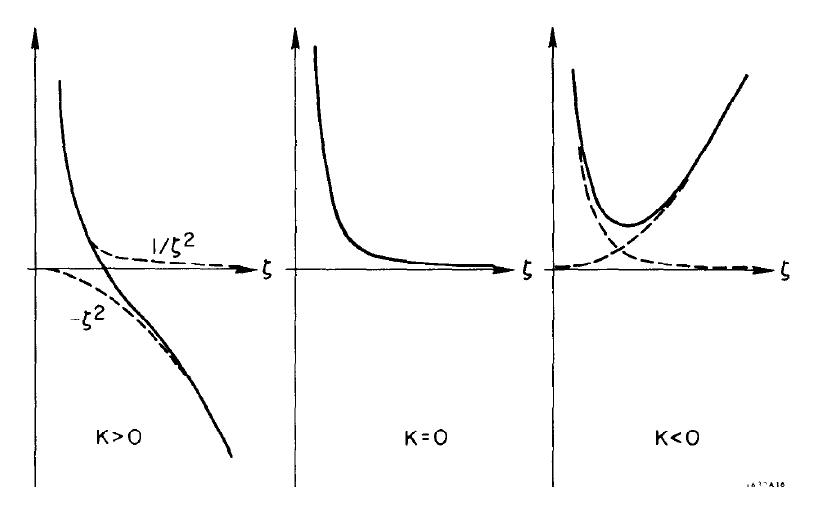
\includegraphics[width=0.8\linewidth]{./Figuras/fig16.jpeg}
	\caption{Effective ``potential'' functions for $\zeta$.}
	\label{fig:fig16}
\end{figure}

It is also qualitatively apparent that there may exist ``stable''  solutions for which $\zeta(s)$ enters a region of $K < 0$ moving inward (toward the origin) and is turned around by the ``repulsion'' only to be sent back inward again by the ``attractive'' force in a later region where $K > 0$. For a periodic $K(s)$ like that in Fig. \ref{fig:fig17}, we must expect a solution $\zeta(s)$ like the one sketched in part (b). The solution exhibits an important general characteristic of the function $\zeta(s)$: its maxima occur in focusing sections - one where $K > 0$ - and its minima occur in defocusing sections - where $K < 0$.

\begin{figure}[!htb]
	\centering
	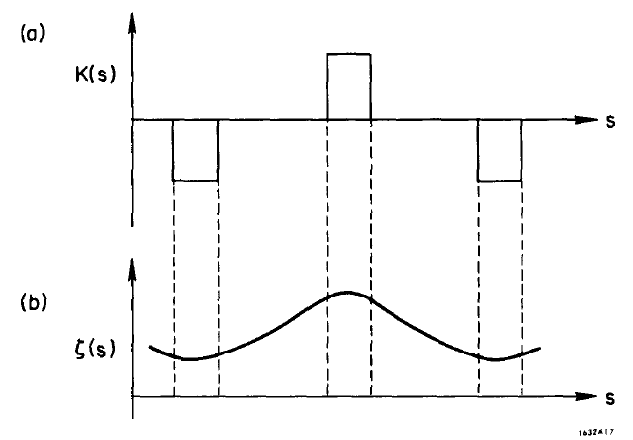
\includegraphics[width=0.8\linewidth]{./Figuras/fig17.jpeg}
	\caption{Form of the function $\zeta(s)$ with a periodic focusing function $K(s)$.}
	\label{fig:fig17}
\end{figure}

It is also clear that, for a given spacing of the segments of different $K$-values, if the magnitude of $K$ is scaled upward, the amplitude of the undulations will grow rapidly larger. Less apparent - and left as a point to ponder - is the fact that as the scale of $K$ is increased a situation will be eventually reached for which a ``stable'' - i.e., periodic - solution no longer exists for $\zeta(s)$. So the strength of the focusing (magnitude of $K$) and the element spacing must be adjusted together in playing with a storage ring \emph{lattice} (a word used to indicate the geometry of the segments).

You may be tempted to wonder: ``Why not just have $K > 0$ at all $s$? Clearly the stability of $\zeta(s)$ is then guaranteed''. But do not forget that when $K$ is positive for one coordinate
 of lateral motion in the storage ring - say $x$ - then the $K$ for the other coordinate - $y$ - is negative, and vice-versa. Recall Eqs. \eqref{eq:2.21} and \eqref{eq:2.22}. The need for an alternating gradient is clear.\\
It should also be now apparent that the undulations of $\zeta(s)$ - and so also of $\beta(s)$ - will be “out-of-phase” in the two coordinates $x$ and $y$, the $\zeta$ for one being at
its maximum where the $\zeta$ for the other is at its minimum.\\
The out-of-phase behavior is quite general - even for rather complicated focusing lattices - although it will not generally be true that the $\zeta_x(s)$ and $\zeta_y(s)$ are entirely
 similar in shape. In Fig. \ref{fig:fig18} I show the two functions $\zeta_x$ and $\zeta_y$ for the periodic lattice of Fig. \ref{fig:fig10}.

\begin{figure}[!htb]
	\centering
	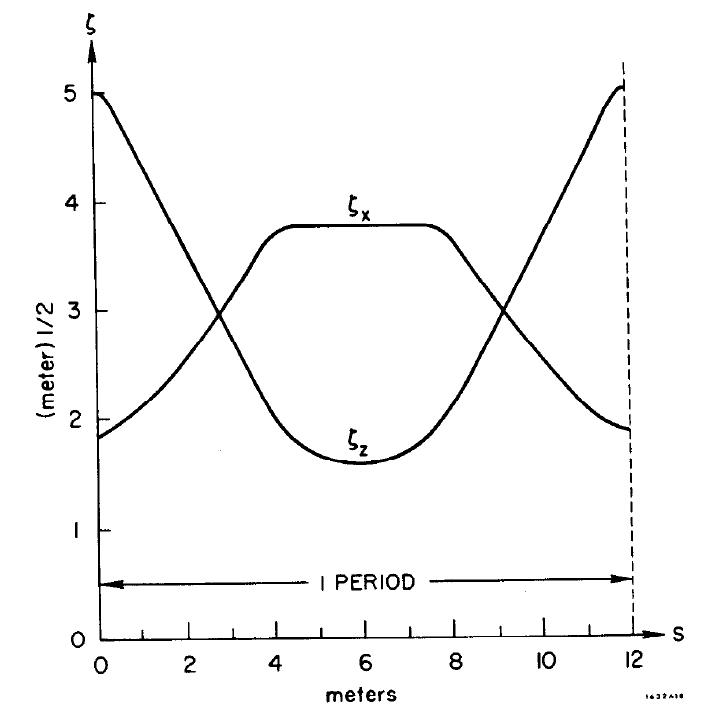
\includegraphics[width=0.8\linewidth]{./Figuras/fig18.jpeg}
	\caption{The functions $\zeta_x$ and $\zeta_y$, for the guide field of Fig. \ref{fig:fig10}.}
	\label{fig:fig18}
\end{figure}

It is instructive to relate the betatron function $\beta(s)$ to the sine-like trajectories which were defined in Section \ref{sec:2.6}. The sine-like trajectory $S(s, s_o)$ associated with the azimuth $s_0$ is that trajectory which starts at so with zero displacement
and unit slope. It can be expressed in terms of the pseudo-harmonic oscillation Eq. \eqref{eq:2.46} by setting $a = \sqrt{\beta(s_0)}$ and $\vartheta = \pi/2+\varphi(s_0)$:
\begin{align}
	S(s,s_0) = \sqrt{\beta(s_0)\beta(s)}\sin\int_{s_0}^s\dfrac{d\bar{s}}{\beta(\bar{s})}.
\end{align}
(You can check that $S(s_0, s_0) = 0$, and $S'(s_0, s_0) = 1$.) Now consider what happens if we follow this sine-like trajectory for one complete revolution - that is to $s = s_0 + L$. The integral becomes, by Eq. \eqref{eq:2.60} just $2\pi\nu$. Because of the periodicity of the betatron function, $\beta(s_0 + L) = \beta(s_0)$. So
\begin{align}
	S(s_0+L,s_0)=\beta(s_0)\sin{(2\pi\nu)}
\end{align}
which - since $\nu$ is independent of $s_0$ - I can also write as

\begin{align}\label{eq:2.77}
	\beta(s)=\dfrac{S(s+L,s)}{\sin{(2\pi\nu)}}.
\end{align}
The betatron-function at $s$ is, within a constant, just the displacement after one revolution
 of the sine-like trajectory which starts at $s$. See Fig. \ref{fig:fig19}.\\
We now have another prescription for finding $\beta(s)$. One needs only calculate directly the sine-like trajectory after one revolution, starting at each $s$.\\
\begin{figure}[!htb]
	\centering
	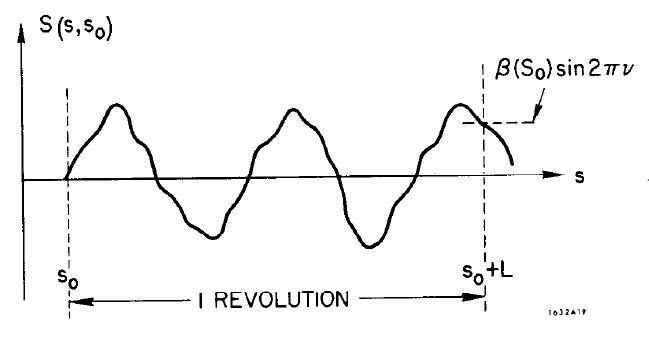
\includegraphics[width=0.8\linewidth]{./Figuras/fig19.jpeg}
	\caption{Relation between $S(s, s_0)$ and $\beta(s_0)$.}
	\label{fig:fig19}
\end{figure}
The displacements obtained are proportional to $\beta(s)$. There is left only to determine the ``normalization'' factor $1/2\pi\nu$. Using the definition of $\nu$, Eq. \eqref{eq:2.60} together with Eq. \eqref{eq:2.77}, you can see that $\nu$ can be obtained as the solution of the transcendental equation
\begin{align}
	\dfrac{2\pi\nu}{\sin{(2\pi\nu)}}=\oint\dfrac{ds}{S(s+L,s)}.
\end{align}
So, given $S(s+L, s)$ for all $s$, we can determine uniquely $\beta(s)$.\\
The calculation of $S(s +L, s)$ can be carried out by a straightforward numerical integration
 of the equations of motion. Or, for a piece-wise-uniform guide field, it is conveniently obtained by using the matrix method described in Section \ref{sec:EqsMotion}. Recalling Eq. \eqref{eq:2.37}, the sine-like trajectory from $s_0$ to $s_0 + L$ is just the upper right element of the transfer matrix $\bm{M}(s, s_0)$ for the complete machine starting at each azimuth $s_0$.\\
It can also be shown - but I shall not stop to do so - that $\nu$ can be obtained from the trace of the matrix for the complete ring. Namely
\begin{align}
	\cos{(2\pi\nu)} &= \dfrac{1}{2}\Tr\bm{M}(s+L,s) \\
    	&= \dfrac{1}{2}\left\lbrace C(s+L,s)+S'(s+L,s) \right\rbrace,
\end{align}
where $C$ is the cosine-like function. So if $C$ and $S'$ are calculated as well as $S$, $\nu$ can be determined and Eq. \eqref{eq:2.77} will give $\beta(s)$ directly.\\
Although I have thought it more convenient to write the differential equation for $\beta$ in terms of its square root $\zeta$, one can, of course, write one in terms of $\beta$ directly. Equation \eqref{eq:2.74} can be rewritten as
\begin{align}\label{eq:2.80}
	\dfrac{1}{2}\beta\beta'' - \dfrac{1}{4}\beta'^2 + K(s)\beta^2 = 1.
\end{align}
The form is clearly less convenient. I may, however, use it to make the following observations.\\
In a field free segment of the guide field $K(s) = 0$, and the solution to Eq. \eqref{eq:2.80} is
\begin{align}\label{eq:2.81}
	\beta = \beta_0 \left\lbrace 1 + \dfrac{(s-s_0)^2}{\beta_0^2} \right\rbrace
\end{align}
where $s_0$ and $\beta_0$ are suitable constants. If $\beta$ has a minimum in the field free segment then $\beta_0$ and $s_0$ are the values of $\beta$ and $s$ at the minimum. Generally, the
intersection of two colliding beams occurs at a symmetry point where $\beta$ must be a minimum. Then Eq. \eqref{eq:2.81} gives the form of $\beta(s)$ in the vicinity of the intersection.

\begin{proof}
	The differential equation we want to solve is
	\begin{align*}
		\frac{1}{2}\beta\beta'' - \left(\frac{\beta'}{2}\right)^2=0
	\end{align*}
	This is a second-order nonlinear ordinary differential equation. It is also an autonomous equation, which means that it does not explicitly contain the independent variable -- in this case, $s$. So, it's possible to treat $\beta$ as the independent variable and define a new variable $\alpha$ given by
	\begin{align*}
		\alpha(\beta) = -\frac{\beta'}{2}
	\end{align*}
	So, we can write
    \begin{align*}
		\beta'' &= -2\frac{d\alpha}{d \beta}\beta' = -2\frac{d\alpha}{d \beta}(-2\alpha) = 4\alpha\frac{d\alpha}{d\beta}
	\end{align*}
	Replacing this in the differential equation:
	\begin{align*}
		2\alpha\beta\frac{d\alpha}{d\beta} &= 1 + \alpha^2\\
		\Rightarrow \frac{2\alpha}{1+\alpha^2}d\alpha &= \frac{1}{\beta}d\beta
	\end{align*}
	Integrating both sides of the equation:
	\begin{align*}
		\int_{\alpha_0}^{\alpha} \frac{2\alpha}{1+\alpha^2}d\alpha &= \int_{\beta_0}^{\beta} \frac{d\beta}{\beta}\\
		\Rightarrow \ln\left(\dfrac{1+\alpha^2}{1+\alpha_0^2}\right) &= \ln\left(\dfrac{\beta}{\beta_0}\right)\\
	\end{align*}
	Then, it is easy to see that
    \begin{align*}
    	\frac{1+\alpha^2}{\beta} = \frac{1+\alpha_0^2}{\beta_0}.
	\end{align*}
	Defining $\gamma_0 = \frac{1+\alpha_0^2}{\beta_0}$, we can rewrite it as
	\begin{align*}
		&\frac{1+\alpha^2}{\beta} = \gamma_0\\
		\Rightarrow & \,\alpha = \sqrt{\beta\gamma_0 -1}
	\end{align*}
	But we know that $\alpha = -\beta'/2$. So,
	\begin{align*}
		-\frac{1}{2}\frac{d\beta}{ds} &= \sqrt{\beta\gamma_0 -1}\\
		\Rightarrow -\frac{d\beta}{2\sqrt{\beta\gamma_0 -1}} &= ds
	\end{align*}
	Integrating both sides of the equation:
	\begin{align*}
		\int\limits_{\beta_0}^{\beta}-\frac{d\beta}{2\sqrt{\beta\gamma_0 -1}} &= \int\limits_{s_0}^{s}ds\\
		\left.\begin{matrix}
		-\frac{1}{\gamma_0}\sqrt{\beta\gamma_0-1}
		\end{matrix}\ \right|^\beta_{\beta_0} &= \left.\begin{matrix}
				s
				\end{matrix}\ \right|^s_{s_0}\\
		\sqrt{\beta_0\gamma_0-1}-\sqrt{\beta\gamma_0-1} &= \gamma_0(s-s_0)
	\end{align*}
	As we said later, $\gamma_0 = \frac{1+\alpha_0^2}{\beta_0}$. So,
	\begin{align*}
		\sqrt{1-\alpha_0^2-1}-\sqrt{\beta\gamma_0-1} &= \gamma_0(s-s_0)\\
		-\alpha_0-\sqrt{\beta\gamma_0-1} &= \gamma_0(s-s_0)\\
		-\sqrt{\beta\gamma_0-1} &= \alpha_0+\gamma_0(s-s_0)\\
	\end{align*}
	We can evaluate the square of the equation and obtain that
	\begin{align*}
		\beta\gamma_0-1 &= [\alpha_0+\gamma_0(s-s_0)]^2\\
		\therefore \beta &= \frac{1}{\gamma_0}[1+(\alpha_0+\gamma_0(s-s_0))^2]
	\end{align*}
	At its minimum, $\beta'=0$ and $\alpha=0$. In this case,
	\begin{align*}
		\beta &= \beta_0\left[1+\frac{1}{\beta_0^2}(s-s_0)^2\right]
	\end{align*}
\end{proof}

Its form is illustrated in Fig. \ref{fig:fig20}. Notice that the coefficient of the quadratic term is just the inverse of the value of $\beta$ at the minimum - the smaller is $\beta_0$, the more rapid the increase of $\beta$ with increasing distance from the minimum.

\begin{figure}[!htb]
	\centering
	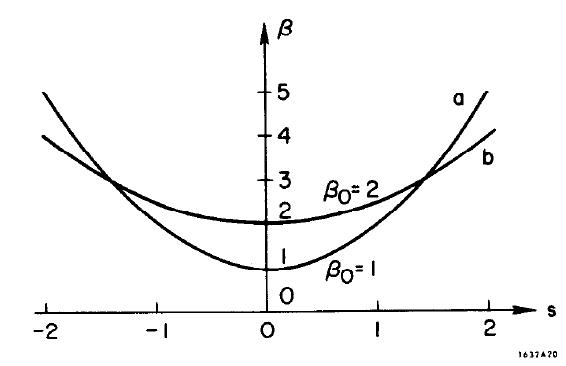
\includegraphics[width=0.8\linewidth]{./Figuras/fig20.jpeg}
	\caption{Variation of $\beta$ near the minimum that occurs in a long field free region.}
	\label{fig:fig20}
\end{figure}

Finally, observe that in a segment in which $K$ is large and $\beta'$ is not, Eq. \eqref{eq:2.80} can be approximated by
\begin{align}
	\beta'' = -2 K \beta.
\end{align}
Then, $\beta$ is a sinusoid or an exponential depending on the sign of $K$.
